\documentclass[conference,a4paper]{IEEEtran}
\IEEEoverridecommandlockouts
\usepackage{cite}
\usepackage{amsmath,amssymb,amsfonts}
\usepackage{algorithmic}
\usepackage{graphicx}
\usepackage{textcomp}
\usepackage{xcolor}
\usepackage{booktabs}
\def\BibTeX{{\rm B\kern-.05em{\sc i\kern-.025em b}\kern-.08em
    T\kern-.1667em\lower.7ex\hbox{E}\kern-.125emX}}

\newcommand{\gmean}{\mbox{G-mean}}

\begin{document}

\title{Explanation-Guided Synthetic Oversampling for Imbalanced Classification}

\author{
\IEEEauthorblockN{Uday Raj}
\IEEEauthorblockA{\textit{Department of Computer Science and Engineering} \\
rajuday6002@gmail.com}
\and
\IEEEauthorblockN{Monika Sharma}
\IEEEauthorblockA{\textit{Department of Computer Science and Engineering} \\
monikasharma6826@gmail.com}
}

\maketitle

\begin{abstract}
Imbalanced classification remains a pervasive challenge in tabular machine learning. While synthetic oversampling techniques like SMOTE balance class proportions, uniform exploration across feature dimensions risks blurring critical decision boundaries. This paper investigates Attribution-Constrained SMOTE (AC-SMOTE), a method leveraging feature attributions to guide synthetic generation. By computing local feature importance from a surrogate model, AC-SMOTE penalizes dissimilarities along high-attribution dimensions during neighbor selection and restricts interpolation along critical minority features. Across a benchmark of 10 datasets and three classifiers, AC-SMOTE demonstrates statistically significant improvements over no resampling on \gmean{} and Balanced Accuracy, achieving the lowest mean rank on unscaled Logistic Regression. However, after rigorous family-wise error rate control via Holm-Bonferroni correction, there is no evidence of benefit over standard SMOTE, Borderline-SMOTE, or SMOTETomek. Furthermore, SHAP-derived attributions show no significant advantage over a uniform attribution control ($p = 1.0$), and uncalibrated oversampling degrades Logistic Regression probability calibration. These findings provide an empirically rigorous, transparent characterization of when and why attribution constraints affect synthetic oversampling.
\end{abstract}

\begin{IEEEkeywords}
Imbalanced Learning, SMOTE, Explainable AI, SHAP, Synthetic Data Generation
\end{IEEEkeywords}

\section{Introduction}
Learning from highly imbalanced datasets is a foundational problem in applied machine learning. When the class of interest (minority class) is heavily outnumbered by the background class (majority class), standard inductive algorithms frequently maximize raw accuracy by trivializing predictions toward the majority class. This behavior is catastrophic in domains such as financial fraud detection, rare disease screening, and equipment fault diagnosis, where false negatives incur substantial penalties.

To mitigate class disparity, data-level interventions such as synthetic oversampling are widely deployed. The Synthetic Minority Over-sampling Technique (SMOTE) \cite{chawla2002smote} synthesizes minority instances through convex linear combinations of neighboring minority samples. Despite its broad adoption, standard SMOTE assumes uniform geometric isotropic exploration: all feature dimensions are weighted equally during both nearest-neighbor retrieval and sample synthesis. In complex, high-dimensional manifolds, unguided interpolation frequently places synthetic points across empirical class boundaries, introducing label noise and distorting downstream classifier margins.

To evaluate whether domain saliency can prevent boundary contamination, this paper examines Attribution-Constrained SMOTE (AC-SMOTE). Rather than treating all coordinate axes identically, AC-SMOTE incorporates Explainable AI (XAI) attributions into the generative mechanism. Local feature importances extracted via TreeExplainer \cite{lundberg2020local} from a surrogate Random Forest are converted into an attribution vector. This vector is applied in two distinct stages: first, weighting the distance metric to ensure nearest neighbors share similarity along salient dimensions; second, contracting the interpolation step size along critical axes to retain fidelity to original minority modes.

The core contributions of this work include:
\begin{enumerate}
\item Formalizing attribution-weighted metric selection and attribution-constrained interpolation within an imbalanced-learn compatible pipeline.
\item Benchmarking AC-SMOTE against seven established baselines across 10 benchmark datasets, three diverse classifiers (Logistic Regression, Random Forest, and XGBoost), and 15 repeated cross-validation folds.
\item Conducting confirmatory statistical testing with Holm-Bonferroni and Benjamini-Hochberg adjustments, combined with boundary fidelity, probability calibration, and attribution ablation studies that transparently delineate the capabilities and empirical boundaries of the approach.
\end{enumerate}

\section{Related Works}
\subsection{Classical and Adaptive Resampling}
Since the development of SMOTE \cite{chawla2002smote}, extensive research has focused on refining sample placement. Borderline-SMOTE \cite{han2005borderline} restricts synthesis to minority instances near the decision frontier based on majority neighbor ratios. ADASYN \cite{he2008adasyn} adaptively allocates synthetic density proportional to local learning difficulty. Safe-level SMOTE, SVM-SMOTE \cite{nguyen2011svm}, and SMOTE-Tomek \cite{batista2004study} further combine spatial filtering with undersampling to purge borderline ambiguities. Additionally, feature-weighted variations such as FW-SMOTE and cluster-based algorithms like K-means SMOTE have explored global feature scaling or clustering centroids prior to oversampling. However, existing methods predominantly focus on sample selection rather than constraining directional interpolation per dimension.

\subsection{Explainable AI in Imbalanced Learning}
Model interpretability techniques, particularly Shapley values via SHAP \cite{lundberg2017unified, lundberg2020local}, have provided rigorous cooperative game-theoretic foundations for attributing individual prediction credit. While attributions have traditionally served post-hoc diagnostic functions, emerging efforts explore integrating explanations into training objectives and data curation. AC-SMOTE tests the hypothesis that directing generation along low-variance, high-importance dimensions preserves boundary geometry under severe skew.

\section{Methods}
\subsection{Algorithmic Formulation}
Let $X \in \mathbb{R}^{n \times d}$ denote training features and $y \in \{0, 1\}^n$ denote binary class labels, with minority subset $X_{min} \subset X$ ($|X_{min}| = n_{min}$) and majority subset $X_{maj}$ ($|X_{maj}| = n_{maj}$). To balance class counts, $n_{syn} = n_{maj} - n_{min}$ instances must be synthesized.

\textbf{Step 1 (Attribution Vector):} A surrogate Random Forest $f_{surr}$ (50 estimators, maximum depth 6) is trained on $(X, y)$. Absolute TreeExplainer SHAP values $\Phi \in \mathbb{R}^{n_{min} \times d}$ are computed across all minority samples. The mean importance vector $w \in \mathbb{R}^d$ is:
\begin{equation}
w_j = \frac{1}{n_{min}} \sum_{i=1}^{n_{min}} |\Phi_{i,j}|
\end{equation}
The vector is min-max scaled to yield normalized feature weights $\hat{w}_j = \frac{w_j - \min(w)}{\max(w) - \min(w) + \epsilon} \in [0, 1]$.

\textbf{Step 2 (Attribution-Weighted Neighbor Selection):} For any pair of minority instances $u, v \in X_{min}$, the attribution-weighted distance is defined as:
\begin{equation}
d_w(u, v) = \sqrt{\sum_{j=1}^d \left( 1 + \alpha \hat{w}_j \right) (u_j - v_j)^2}
\end{equation}
where $\alpha \geq 0$ scales distance along critical dimensions (default $\alpha = 2.0$). The $k$ nearest minority neighbors under $d_w$ are indexed for each instance.

\textbf{Step 3 (Attribution-Constrained Interpolation):} To synthesize a new sample from minority base point $x_i$ and neighbor $x_{nn}$, a standard random scalar $\lambda \sim U(0, 1)$ is scaled feature-wise:
\begin{equation}
\lambda_j = \max\left(0, \min\left(1, \lambda \times (1 - \beta \hat{w}_j) \right)\right)
\end{equation}
where $\beta \in [0, 1]$ dictates contraction strength (default $\beta = 0.7$). The resulting synthetic point is formed coordinate-wise:
\begin{equation}
x_{synth, j} = x_{i, j} + \lambda_j (x_{nn, j} - x_{i, j})
\end{equation}

\subsection{Experimental Design and Evaluation Protocol}
Experiments encompass 10 benchmark datasets spanning diverse imbalance ratios ($IR$) and feature dimensions (Table \ref{tab:datasets}). Eight datasets originate from the standard \textit{imbalanced-learn} repository \cite{lemaitre2017imbalanced}, and two real-world datasets (\textit{creditcard} fraud and \textit{telco\_churn}) are sourced from Kaggle.

To prevent data leakage, 5-fold cross-validation with 3 repeats (15 folds total) is executed. All scaling, imputation, surrogate training, and oversampling operations occur strictly inside each training fold. Three downstream classifiers are evaluated: Logistic Regression (LR), Random Forest (RF, 100 trees), and XGBoost (XGB, 100 trees). Five performance metrics are tracked: F1-score, Area Under Precision-Recall Curve (AUC-PR), Matthews Correlation Coefficient (MCC), Geometric Mean (\gmean{}), and Balanced Accuracy.

\textbf{Implementation and Preprocessing Constraints:} For SVMSMOTE and SMOTETomek, majority class training samples are capped at 20,000 to maintain computational tractability (binding exclusively for \textit{creditcard}; in boundary fidelity, memory limits necessitated a 2,000 cap on select runs with $<0.001$ effect on mean rank correlation). In probability calibration evaluation, \textit{creditcard} is excluded because a stratified subsample yields too few positive cases ($\approx 26$) to estimate stable calibration curves.

\begin{table}[htbp]
\caption{Benchmark Dataset Characteristics}
\label{tab:datasets}
\centering
\begin{tabular}{lrrrrr}
\toprule
\textbf{Dataset} & \textbf{Samples} & \textbf{Features} & \textbf{Minority} & \textbf{Majority} & \textbf{IR} \\
\midrule
ecoli & 336 & 7 & 35 & 301 & 8.60 \\
satimage & 6,435 & 36 & 626 & 5,809 & 9.28 \\
spectrometer & 531 & 93 & 45 & 486 & 10.80 \\
car\_eval\_34 & 1,728 & 21 & 134 & 1,594 & 11.90 \\
oil & 937 & 49 & 41 & 896 & 21.85 \\
wine\_quality & 4,898 & 11 & 183 & 4,715 & 25.77 \\
mammography & 11,183 & 6 & 260 & 10,923 & 42.01 \\
abalone\_19 & 4,177 & 10 & 32 & 4,145 & 129.53 \\
creditcard & 284,807 & 29 & 492 & 284,315 & 577.88 \\
telco\_churn & 7,043 & 30 & 1,869 & 5,174 & 2.77 \\
\bottomrule
\end{tabular}
\end{table}

\textbf{Hypothesis Testing Protocol:} Confirmatory evaluation uses non-parametric Friedman tests across the 8 resampling treatments followed by two-sided Wilcoxon signed-rank tests against AC-SMOTE. The hypothesis testing family is defined per classifier-metric pair across the 7 baseline comparisons ($m = 7$). Family-wise error rate (FWER) is controlled via Holm-Bonferroni \cite{holm1979simple}, while false discovery rate (FDR) is tracked via Benjamini-Hochberg \cite{benjamini1995controlling}. Secondary evaluations (boundary fidelity, calibration, tuning) use directed one-sided tests.

\section{Results and Discussion}
\subsection{Confirmatory Benchmark Results}
Mean ranks across all 10 datasets and 8 resampling approaches are presented in Table \ref{tab:mean_ranks}. Friedman tests indicate significant performance differences across methods for \gmean{} ($\chi^2 = 25.39$ for LR, $\chi^2 = 32.71$ for RF, $\chi^2 = 26.73$ for XGB; all $p < 0.001$). 

\begin{table*}[htbp]
\caption{Mean Ranks of Resampling Methods Across All 10 Datasets (Lower is Better)}
\label{tab:mean_ranks}
\centering
\begin{tabular}{llccccc}
\toprule
Classifier & Method & F1-Score & AUC-PR & MCC & G-Mean & Bal. Acc \\
\midrule
Logistic Regression & None & 5.00 & 3.60 & 4.70 & 7.60 & 7.60 \\
 & ROS & 5.70 & 5.50 & 5.60 & 3.90 & 3.70 \\
 & SMOTE & 3.70 & 3.70 & 3.80 & 3.70 & 3.60 \\
 & B-SMOTE & 5.20 & 6.50 & 5.40 & 5.50 & 5.60 \\
 & ADASYN & 6.20 & 5.70 & 6.10 & 4.70 & 4.90 \\
 & SVMSMOTE & \textbf{2.40} & 4.10 & \textbf{2.70} & 4.20 & 4.00 \\
 & SMOTETomek & 3.40 & \textbf{3.00} & 3.50 & 3.40 & 3.60 \\
 & AC-SMOTE & 4.40 & 3.90 & 4.20 & \textbf{3.00} & \textbf{3.00} \\
\midrule
Random Forest & None & 6.40 & 3.70 & 5.70 & 7.80 & 7.70 \\
 & ROS & 4.50 & \textbf{3.20} & 4.00 & 5.70 & 5.70 \\
 & SMOTE & \textbf{3.50} & 4.00 & \textbf{3.60} & 3.30 & 3.30 \\
 & B-SMOTE & 4.30 & 6.20 & 4.50 & 5.40 & 5.60 \\
 & ADASYN & 5.20 & 5.50 & 5.70 & 3.90 & 3.90 \\
 & SVMSMOTE & 3.70 & 4.10 & 3.80 & 3.30 & 3.20 \\
 & SMOTETomek & 3.80 & 4.80 & 4.00 & \textbf{2.90} & \textbf{2.70} \\
 & AC-SMOTE & 4.60 & 4.50 & 4.70 & 3.70 & 3.90 \\
\midrule
XGBoost & None & 6.20 & 4.30 & 5.40 & 8.00 & 7.60 \\
 & ROS & 4.20 & 4.80 & 4.10 & 5.10 & 5.10 \\
 & SMOTE & \textbf{3.70} & 4.30 & \textbf{4.00} & 3.60 & 3.80 \\
 & B-SMOTE & 3.80 & 5.50 & 4.10 & 4.20 & 4.20 \\
 & ADASYN & 4.70 & 5.70 & 5.00 & 4.00 & 4.00 \\
 & SVMSMOTE & 4.20 & \textbf{3.20} & 4.20 & 3.70 & 3.70 \\
 & SMOTETomek & 4.60 & 4.40 & 4.90 & \textbf{3.30} & \textbf{3.20} \\
 & AC-SMOTE & 4.60 & 3.80 & 4.30 & 4.10 & 4.40 \\
\bottomrule
\end{tabular}
\end{table*}

\begin{figure}[htbp]
\centerline{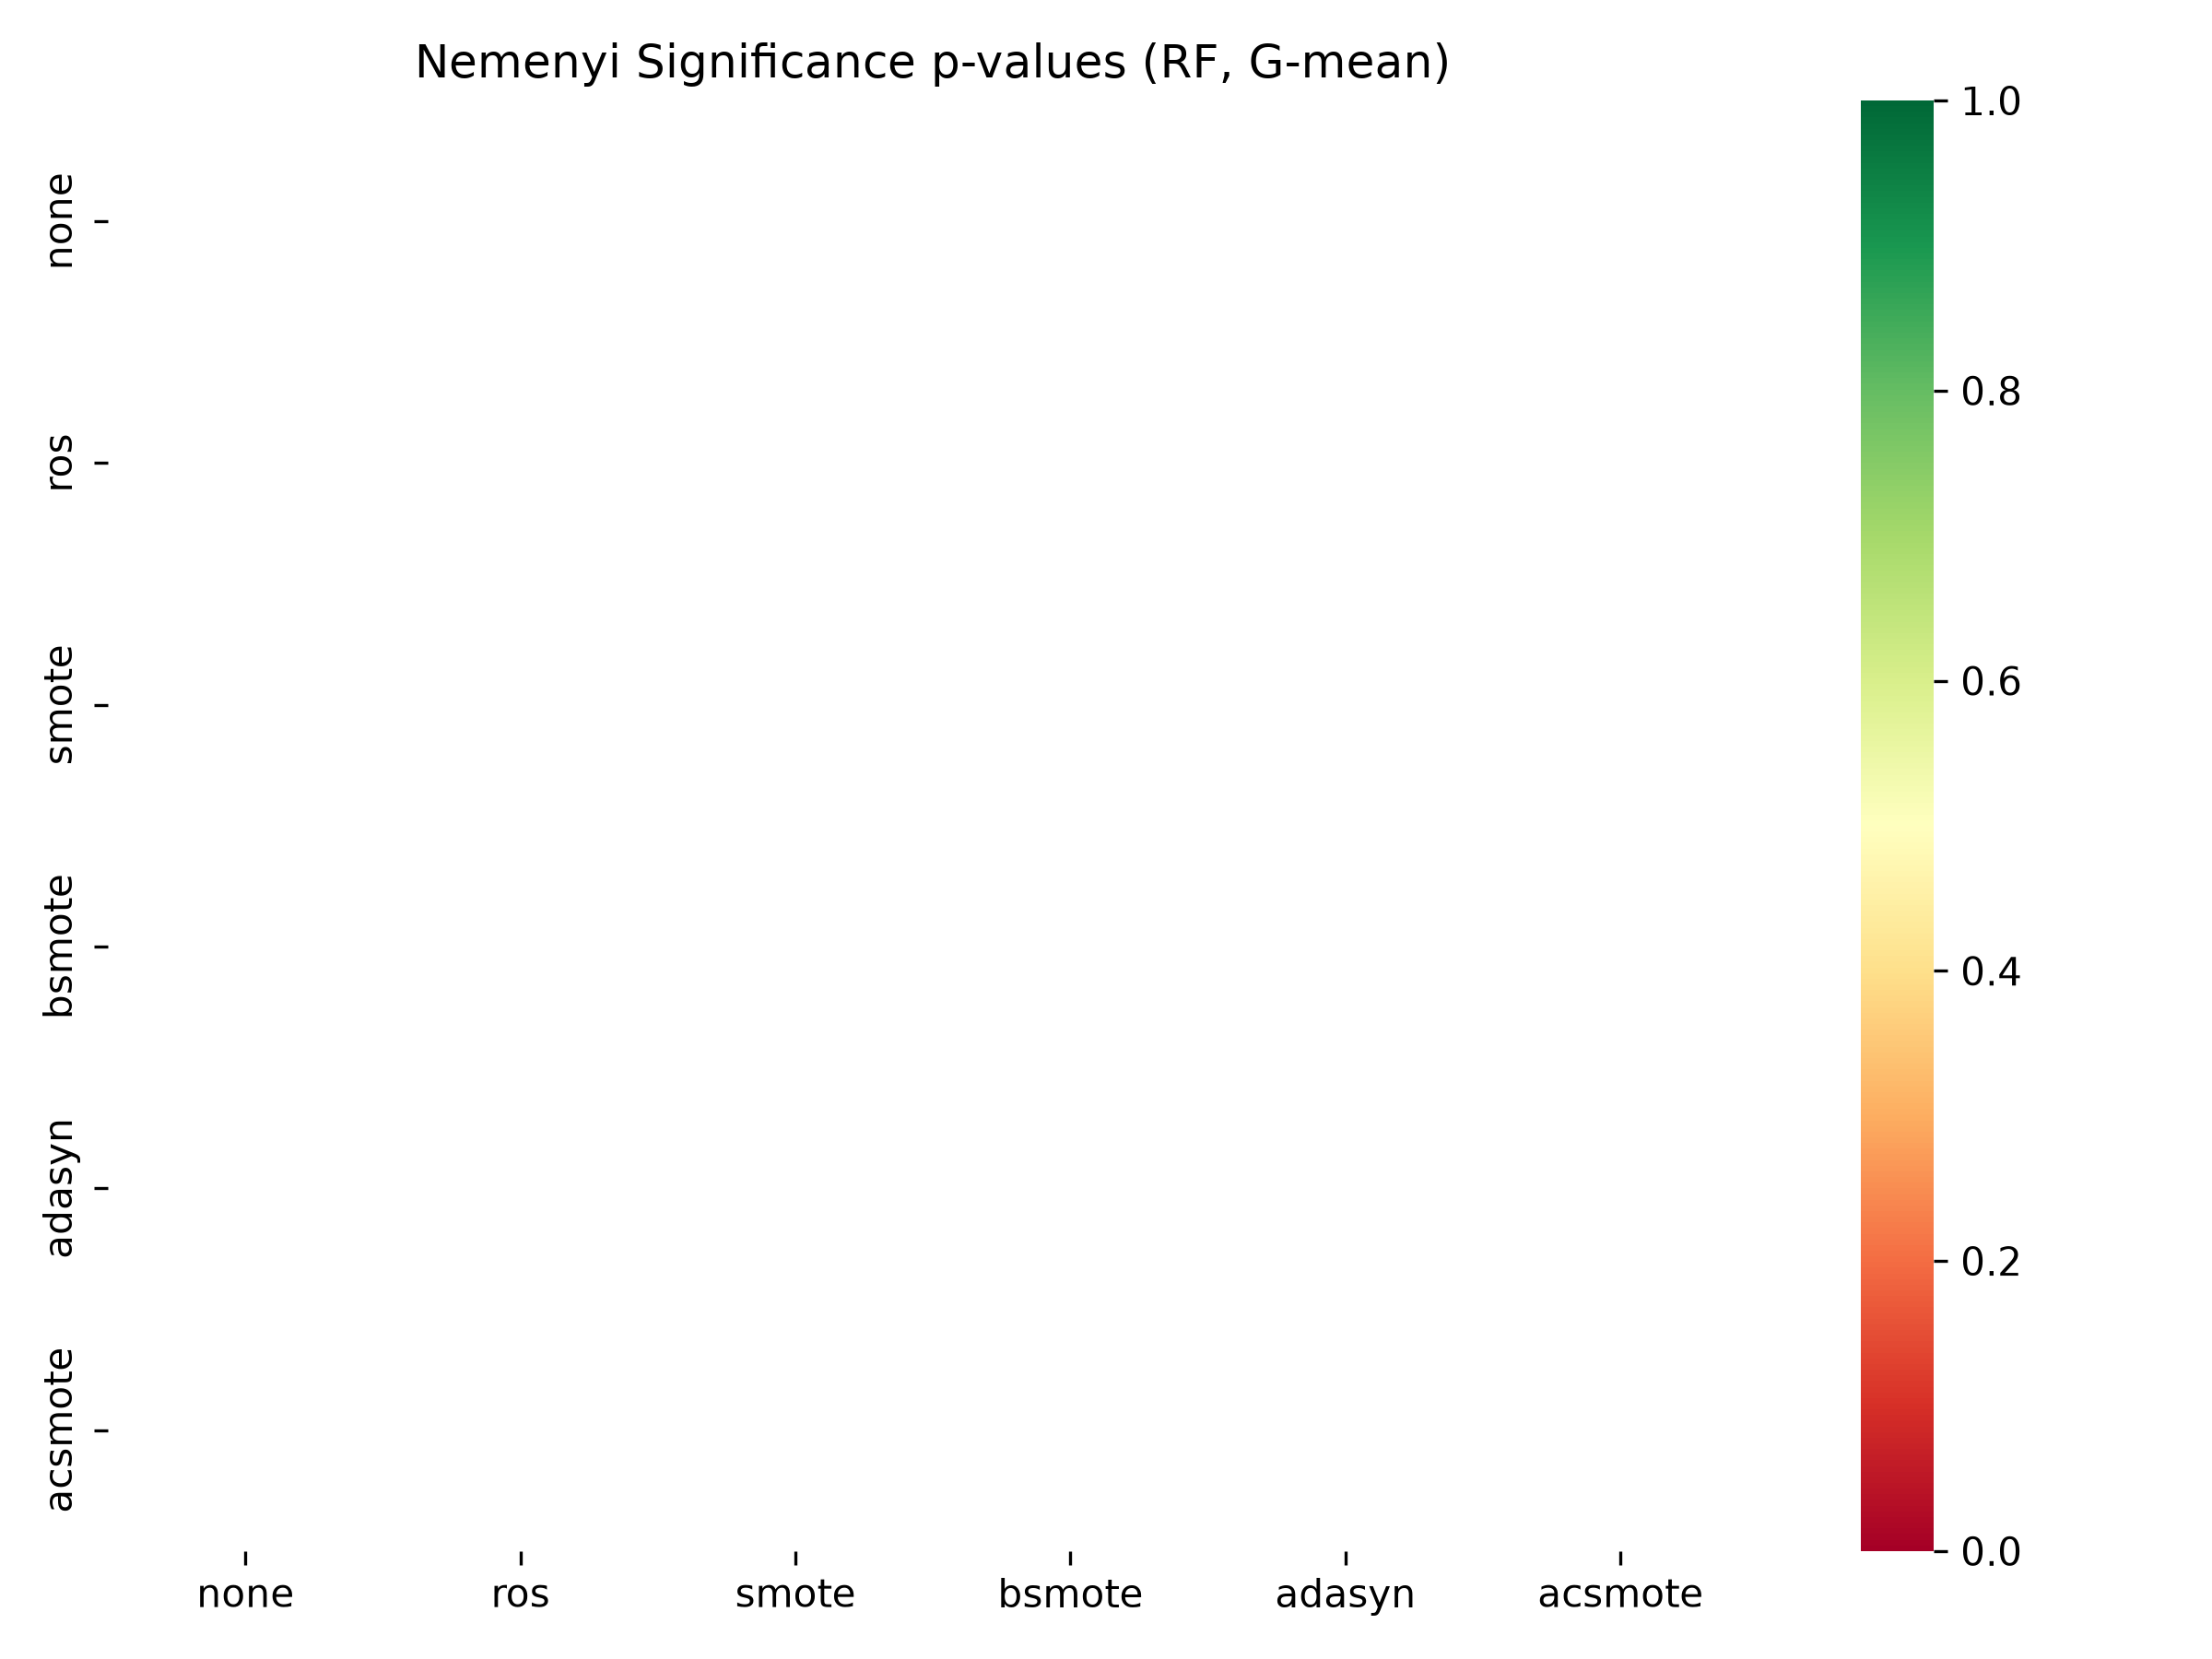
\includegraphics[width=\columnwidth]{figures/critical_difference_diagram.png}}
\caption{Critical difference diagram under Nemenyi post-hoc testing for Random Forest on \gmean{}.}
\label{fig:cd}
\end{figure}

In pairwise Wilcoxon testing against AC-SMOTE:
\begin{itemize}
\item \textbf{Comparison to No Resampling:} AC-SMOTE significantly outperforms `None' on \gmean{} and Balanced Accuracy across all three classifiers (Holm-corrected $p \in [0.014, 0.027]$, winning 9--10 of 10 datasets).
\item \textbf{Comparison to ADASYN:} Under XGBoost, AC-SMOTE significantly improves AUC-PR over ADASYN (Holm-corrected $p = 0.027$, winning 9 of 10 datasets).
\item \textbf{Comparison to Established SMOTE Variants:} Following Holm-Bonferroni correction, there is no evidence of benefit over standard SMOTE, Borderline-SMOTE, or SMOTETomek across any classifier-metric combination.
\item \textbf{Comparison to SVMSMOTE:} On unscaled Logistic Regression F1-score, AC-SMOTE is inferior to SVMSMOTE (1 win, 9 losses; mean F1 0.424 vs. 0.451), statistically significant under BH-FDR ($p = 0.046$) but not Holm.
\end{itemize}

\subsection{Exploratory Analyses: Standardization and Cost Sensitivity}
In exploratory runs where Logistic Regression features were standardized with StandardScaler, raw-feature advantages for SVMSMOTE disappeared, with resamplers clustering within narrow error margins. Similarly, cost-sensitive learning evaluations revealed modest F1/MCC gains for AC-SMOTE on Logistic Regression that survived only under false discovery rate control (BH-FDR $p = 0.0488$), with no significant difference surviving Holm FWER control.

\subsection{Ablation and Boundary Fidelity Studies}
Parameter sweeps over $\beta \in [0, 1]$ on XGBoost (Fig. \ref{fig:ablation}) demonstrate stable performance across non-zero values, with mean \gmean{} moving only modestly (0.715 at $\beta = 0$ to 0.724 at $\beta = 0.7$). However, when evaluating surrogate attribution sources, SHAP guidance does not significantly outperform an uninformative uniform attribution control (pooled $p = 1.0$; \textit{abalone\_19} $p = 0.214$). Simpler attribution heuristics (e.g., Gini impurity or ANOVA F-values) achieve equivalent empirical performance at a fraction of the computational expense.

\begin{figure}[htbp]
\centerline{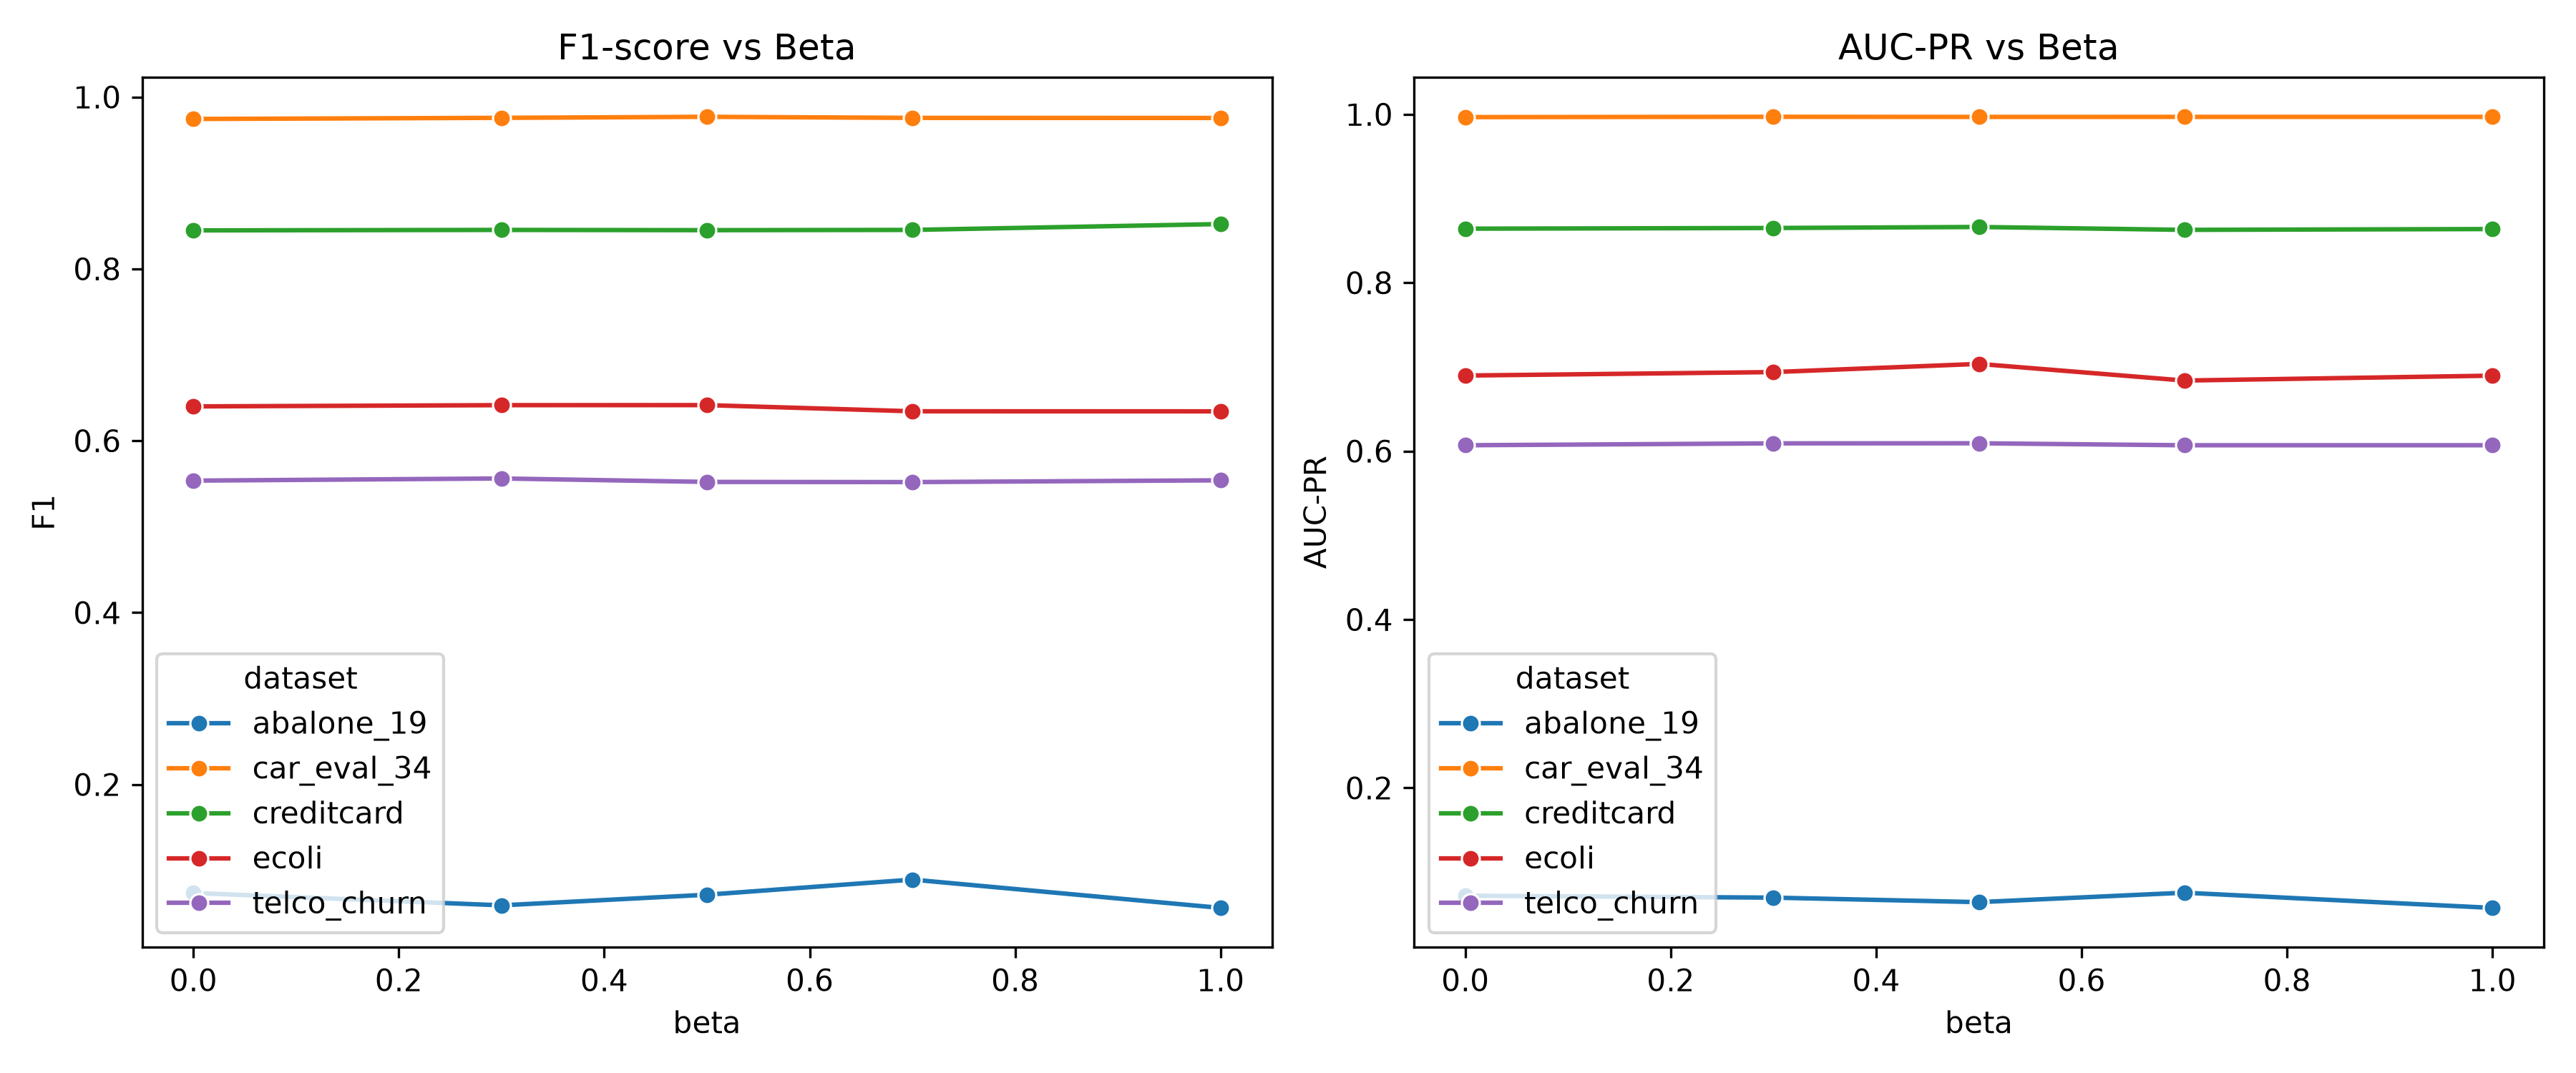
\includegraphics[width=\columnwidth]{figures/ablation_beta_sweep.png}}
\caption{Ablation sweep across interpolation parameter $\beta$ on XGBoost.}
\label{fig:ablation}
\end{figure}

\begin{figure}[htbp]
\centerline{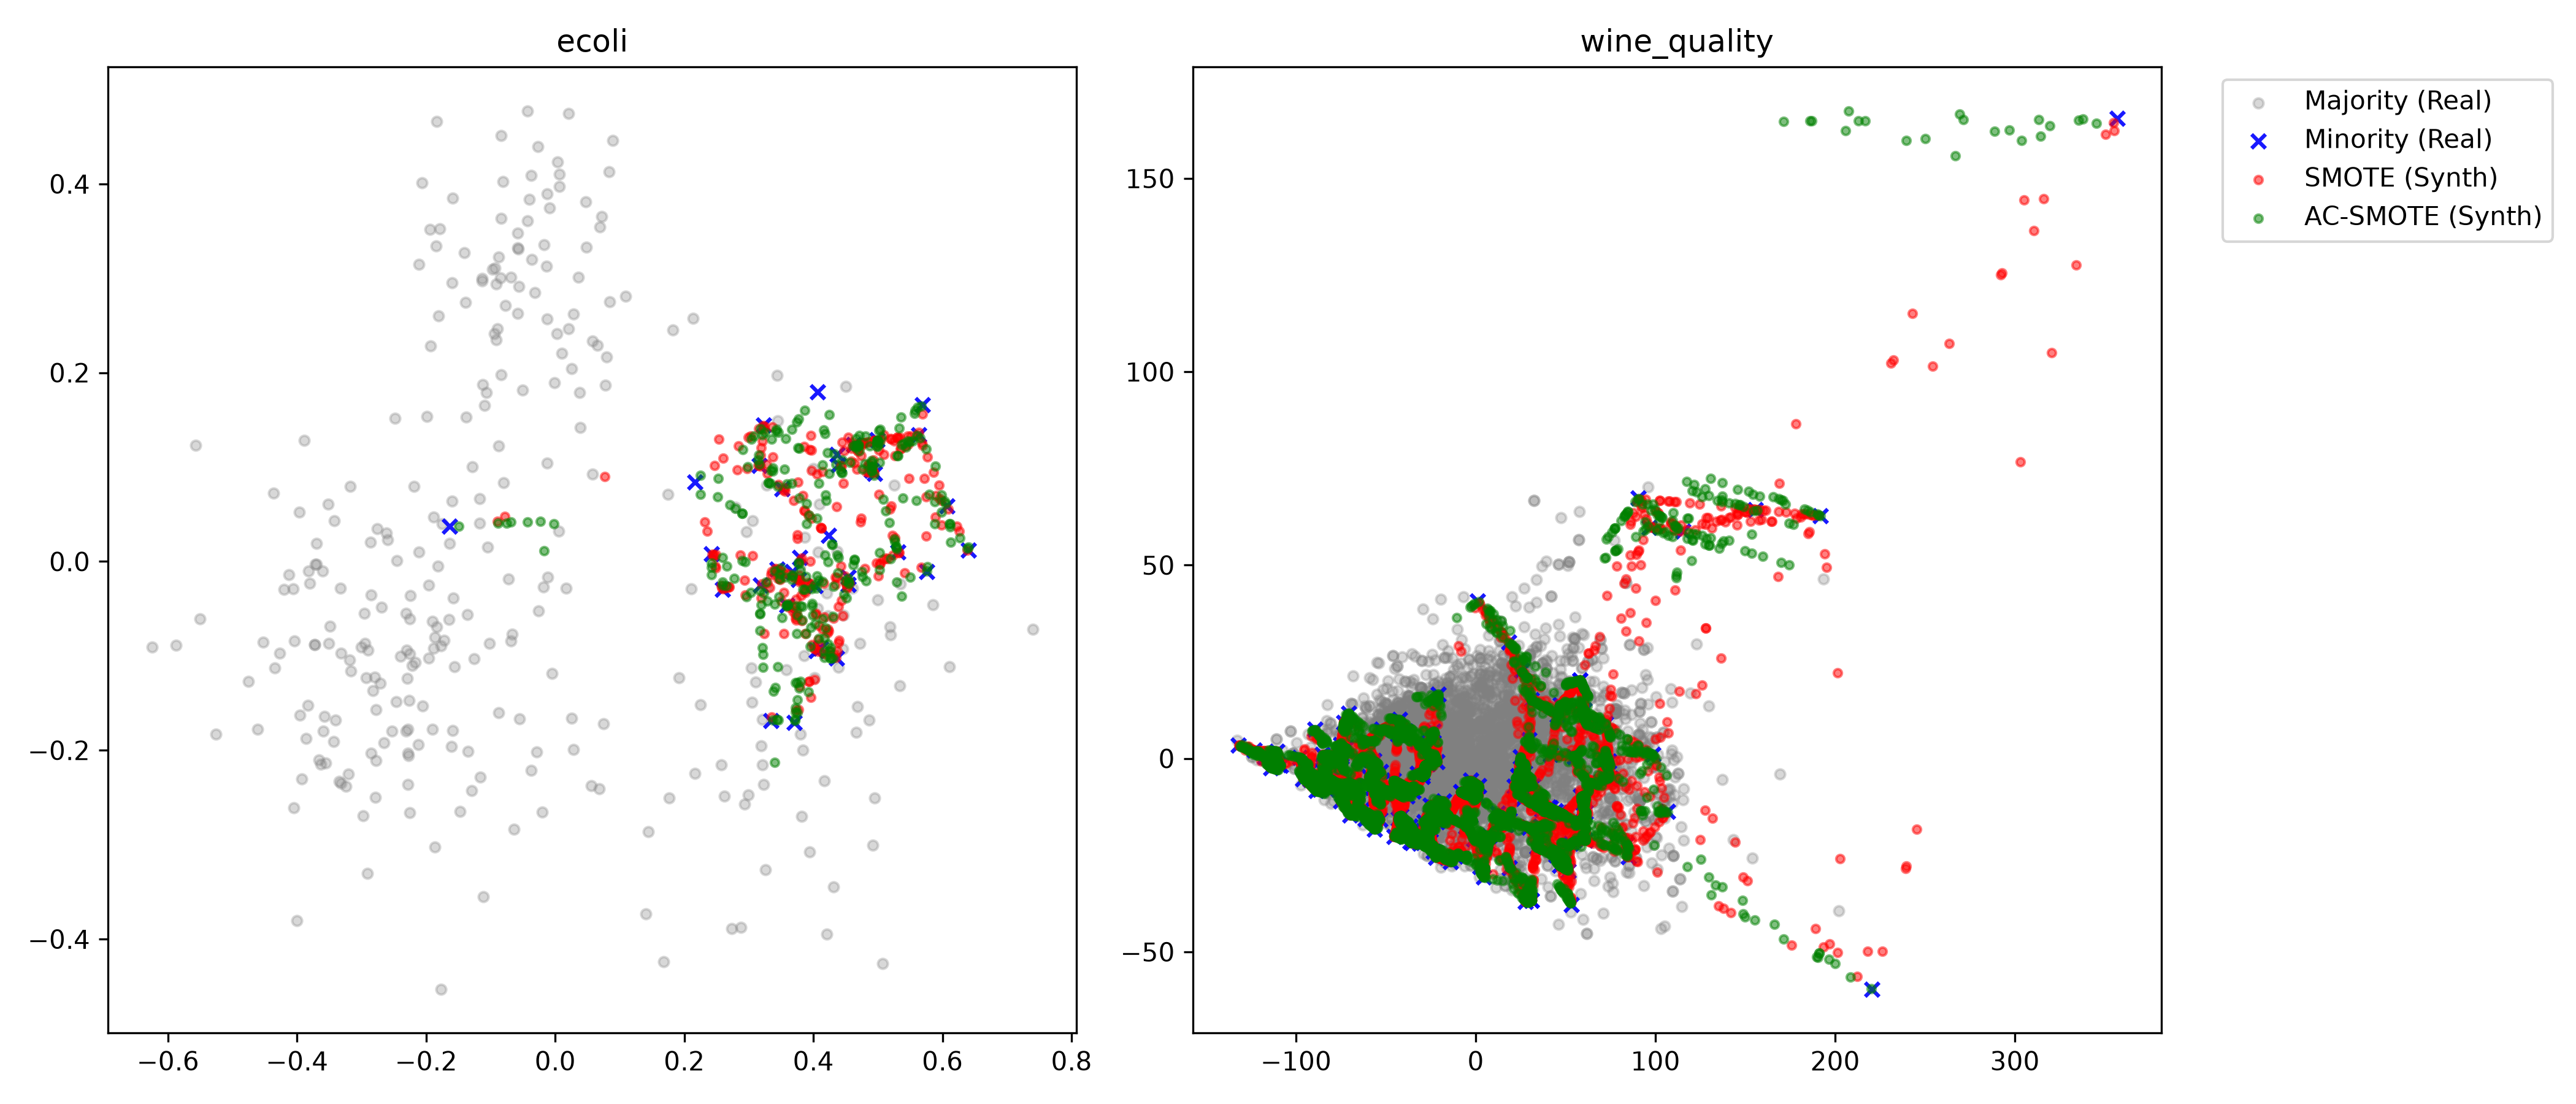
\includegraphics[width=\columnwidth]{figures/pca_synthetic_comparison.png}}
\caption{Two-dimensional PCA projection comparing standard SMOTE and AC-SMOTE synthetic samples.}
\label{fig:pca}
\end{figure}

Boundary fidelity tests measuring Spearman rank correlation between reference test SHAP attributions and post-resampling model attributions showed Random Over-Sampling (ROS) attained the highest boundary preservation (RF 0.807, XGB 0.778). AC-SMOTE achieved comparable fidelity to SMOTE (0.725 vs. 0.729 on RF; 0.632 vs. 0.630 on XGB). A tentative raw gain over ADASYN on RF fidelity ($p = 0.0098$) failed to achieve significance after Holm correction ($p = 0.0586$).

Furthermore, probability calibration analysis revealed that AC-SMOTE, like other synthetic generators, degrades posterior probabilities for Logistic Regression, elevating the Brier score from 0.042 (unresampled baseline) to 0.085.

\begin{figure}[htbp]
\centerline{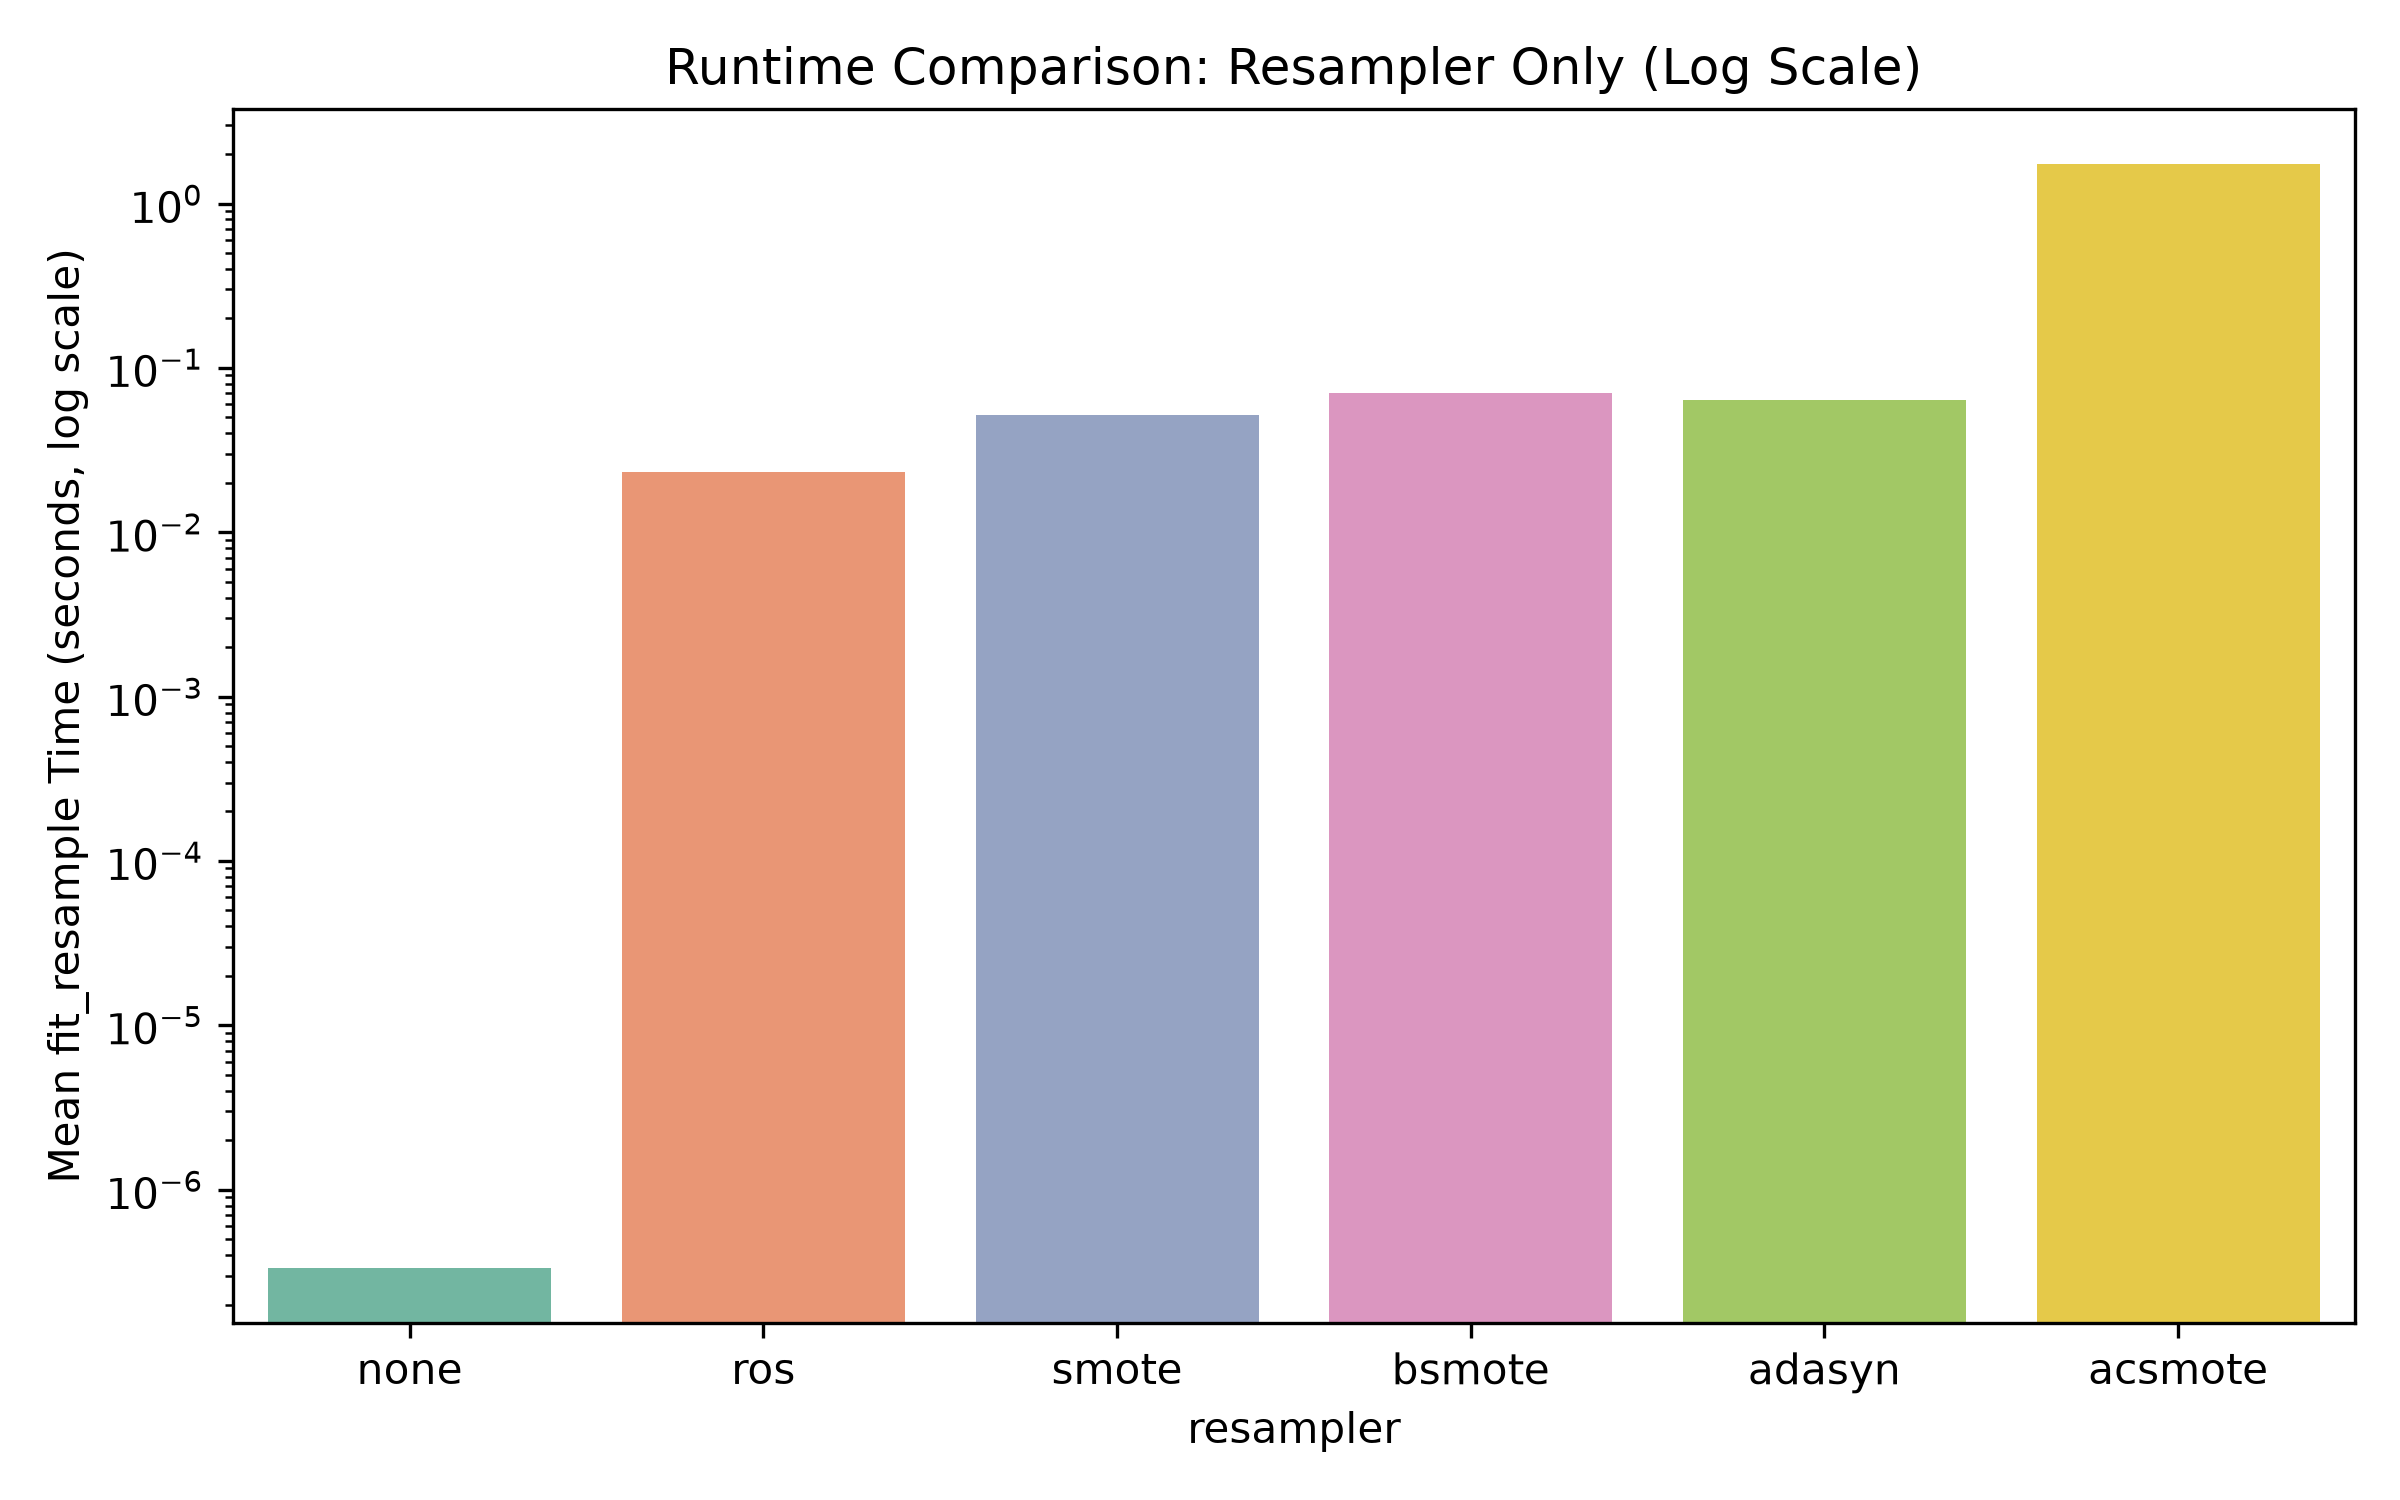
\includegraphics[width=\columnwidth]{figures/runtime_comparison.png}}
\caption{Runtime comparison (seconds, log scale) across resamplers.}
\label{fig:runtime}
\end{figure}

\subsection{Computational Overhead}
As illustrated in Fig. \ref{fig:runtime}, computing TreeExplainer Shapley values over training folds introduces tangible runtime costs compared to nearest-neighbor lookup alone. While AC-SMOTE is considerably faster than SVMSMOTE or SMOTETomek on massive datasets like \textit{creditcard} due to vectorized minority-only calculations, standard SMOTE remains orders of magnitude faster on medium-sized sets.

\subsection{Limitations}
Several methodological limitations must be highlighted:
\begin{enumerate}
\item \textbf{Unweighted Surrogate Modeling:} The initial surrogate Random Forest is trained on raw, imbalanced data without sample weighting, meaning initial SHAP attributions themselves reflect majority-class predictive patterns.
\item \textbf{Normalization Sensitivity:} Min-max scaling of the attribution vector $\hat{w}$ can amplify noise in datasets with near-uniform feature importance distributions.
\item \textbf{Omission of Specialized Baselines:} Highly specialized feature-weighted SMOTE variants (e.g., FW-SMOTE) and cluster-guided variants (e.g., K-means SMOTE) were not benchmarked.
\item \textbf{Asymmetric Tuning and Fixed Thresholds:} Grid tuning was performed primarily on AC-SMOTE hyperparameters rather than joint baseline optimization, and classification metrics were evaluated at default 0.5 decision thresholds rather than threshold-tuned operating points.
\end{enumerate}

\section{Conclusion}
This work evaluated Attribution-Constrained SMOTE (AC-SMOTE), investigating whether Explainable AI attributions can protect decision boundary integrity during synthetic oversampling. A rigorous 15-fold cross-validation benchmark across 10 datasets demonstrates that while AC-SMOTE reliably improves geometry-sensitive metrics over no resampling, there is no evidence of benefit over established methods such as SMOTE, Borderline-SMOTE, and SMOTETomek under formal family-wise error rate control. Furthermore, SHAP attributions perform comparably to uniform attribution baselines, and probability calibration is degraded. These findings underscore the necessity of rigorous, corrected statistical benchmarks in imbalanced learning, revealing that geometric boundary constraints do not automatically translate into downstream classification gains.

\begin{thebibliography}{00}
\bibitem{chawla2002smote} N. V. Chawla, K. W. Bowyer, L. O. Hall, and W. P. Kegelmeyer, ``SMOTE: Synthetic minority over-sampling technique,'' \textit{Journal of Artificial Intelligence Research}, vol. 16, pp. 321--357, 2002.
\bibitem{han2005borderline} H. Han, W.-Y. Wang, and B.-H. Mao, ``Borderline-SMOTE: a new over-sampling method in imbalanced data sets learning,'' in \textit{Advances in Intelligent Computing}, 2005, pp. 878--887.
\bibitem{he2008adasyn} H. He, Y. Bai, E. A. Garcia, and S. Li, ``ADASYN: Adaptive synthetic sampling approach for imbalanced learning,'' in \textit{IEEE International Joint Conference on Neural Networks}, 2008, pp. 1322--1328.
\bibitem{nguyen2011svm} H. M. Nguyen, E. W. Cooper, and K. Kamei, ``Borderline over-sampling for imbalanced data classification,'' \textit{International Journal of Knowledge Engineering and Soft Data Paradigms}, vol. 3, no. 1, pp. 4--21, 2011.
\bibitem{batista2004study} G. E. Batista, R. C. Prati, and M. C. Monard, ``A study of the behavior of several methods for balancing machine learning training data,'' \textit{ACM SIGKDD Explorations Newsletter}, vol. 6, no. 1, pp. 20--29, 2004.
\bibitem{he2009learning} H. He and E. A. Garcia, ``Learning from imbalanced data,'' \textit{IEEE Transactions on Knowledge and Data Engineering}, vol. 21, no. 9, pp. 1263--1284, 2009.
\bibitem{fernandez2018smote} A. Fernandez, S. Garcia, F. Herrera, and N. V. Chawla, ``SMOTE for learning from imbalanced data: progress and challenges, marking the 15-year anniversary,'' \textit{Journal of Artificial Intelligence Research}, vol. 61, pp. 863--905, 2018.
\bibitem{kovacs2019empirical} G. Kovacs, ``An empirical comparison and evaluation of minority oversampling techniques on a large number of imbalanced datasets,'' \textit{Applied Soft Computing}, vol. 83, p. 105662, 2019.
\bibitem{lemaitre2017imbalanced} G. Lemaitre, F. Nogueira, and C. K. Aridas, ``Imbalanced-learn: A python toolbox to tackle the curse of imbalanced datasets in machine learning,'' \textit{Journal of Machine Learning Research}, vol. 18, no. 1, pp. 559--563, 2017.
\bibitem{lundberg2017unified} S. M. Lundberg and S.-I. Lee, ``A unified approach to interpreting model predictions,'' in \textit{Advances in Neural Information Processing Systems}, 2017, pp. 4765--4774.
\bibitem{lundberg2020local} S. M. Lundberg et al., ``From local explanations to global understanding with explainable AI for trees,'' \textit{Nature Machine Intelligence}, vol. 2, no. 1, pp. 56--67, 2020.
\bibitem{chen2016xgboost} T. Chen and C. Guestrin, ``XGBoost: A scalable tree boosting system,'' in \textit{Proceedings of the 22nd ACM SIGKDD International Conference on Knowledge Discovery and Data Mining}, 2016, pp. 785--794.
\bibitem{breiman2001random} L. Breiman, ``Random forests,'' \textit{Machine Learning}, vol. 45, no. 1, pp. 5--32, 2001.
\bibitem{demsar2006statistical} J. Demsar, ``Statistical comparisons of classifiers over multiple data sets,'' \textit{Journal of Machine Learning Research}, vol. 7, pp. 1--30, 2006.
\bibitem{holm1979simple} S. Holm, ``A simple sequentially rejective multiple test procedure,'' \textit{Scandinavian Journal of Statistics}, vol. 6, no. 2, pp. 65--70, 1979.
\bibitem{benjamini1995controlling} Y. Benjamini and Y. Hochberg, ``Controlling the false discovery rate: a practical and powerful approach to multiple testing,'' \textit{Journal of the Royal Statistical Society: Series B (Methodological)}, vol. 57, no. 1, pp. 289--300, 1995.
\bibitem{elkan2001foundations} C. Elkan, ``The foundations of cost-sensitive learning,'' in \textit{International Joint Conference on Artificial Intelligence}, vol. 17, 2001, pp. 973--978.
\bibitem{guo2017calibration} C. Guo, G. Pleiss, Y. Sun, and K. Q. Weinberger, ``On calibration of modern neural networks,'' in \textit{International Conference on Machine Learning}, 2017, pp. 1321--1330.
\end{thebibliography}

\end{document}
